\documentclass[titlepage,a4paper,oneside]{article}
\usepackage[utf8]{inputenc}
\usepackage{amsmath}
\usepackage{mathabx}
\usepackage{graphicx}
\usepackage{minted}
\usepackage{booktabs}
\usepackage[english,spanish,es-noindentfirst,es-nosectiondot,es-nolists,
es-noshorthands,es-lcroman,es-tabla]{babel}
\usepackage{lmodern}             % Use Latin Modern fonts
\usepackage[T1]{fontenc}         % Better output when a diacritic/accent is used
\usepackage[utf8]{inputenc}      % Allows to input accented characters
\usepackage{textcomp}            % Avoid conflicts with siunitx and microtype
\usepackage{microtype}           % Improves justification and typography
\usepackage[svgnames]{xcolor}    % Svgnames option loads navy (blue) colour
\usepackage[hidelinks,urlcolor=blue]{hyperref}
\hypersetup{colorlinks=true, allcolors=Navy, pdfstartview={XYZ null null 1}}
\newtheorem{lemma}{Lema}
\usepackage[width=14cm,left=3.5cm,marginparwidth=3cm,marginparsep=0.35cm,
height=21cm,top=3.7cm,headsep=1cm, headheight=1.6cm,footskip=1.2cm]{geometry}
\usepackage{csquotes}
\usepackage{biblatex}
\addbibresource{informe.bib}
\usepackage[pdf]{graphviz}


\begin{document}

\begin{titlepage}
\title{
	75.74 \-- Distribuidos I \-- TP2\\
    \large Facultad de Ingeniería\\
	Universidad de Buenos Aires
}
\author{
	Mermet, Ignacio Javier\\
	\texttt{98153}
}
\date{Mayo 2022}

\maketitle

\end{titlepage}

\tableofcontents

\newpage

\section{Sobre la entrega}
El código de la entrega se puede encontrar en \href{https://github.com/CrossNox/7574-TP2}{GitHub}.

\section{Estructura del proyecto}
El proyecto fue desarrollado en \texttt{python}\cite{Python} y empaquetado con \texttt{poetry}\cite{PythonPoetry}. Tiene dos CLIs asociadas:

\begin{itemize}
	\item \texttt{rma}:
	\item \texttt{rma\_client}:
\end{itemize}

En la carpeta \texttt{docker} se encuentra disponibles el \texttt{Dockerfile} asociado al paquete.

\section{Instalación y ejecución}
Referirse al archivo \texttt{README.md} provisto en el repositorio para ver las instrucciones de instalación.

\section{DAG}
Pensar tareas que conceptualmente hacen lo mismo, en lugar de tareas que reciben el mismo input.

\begin{figure}[H]
\centering
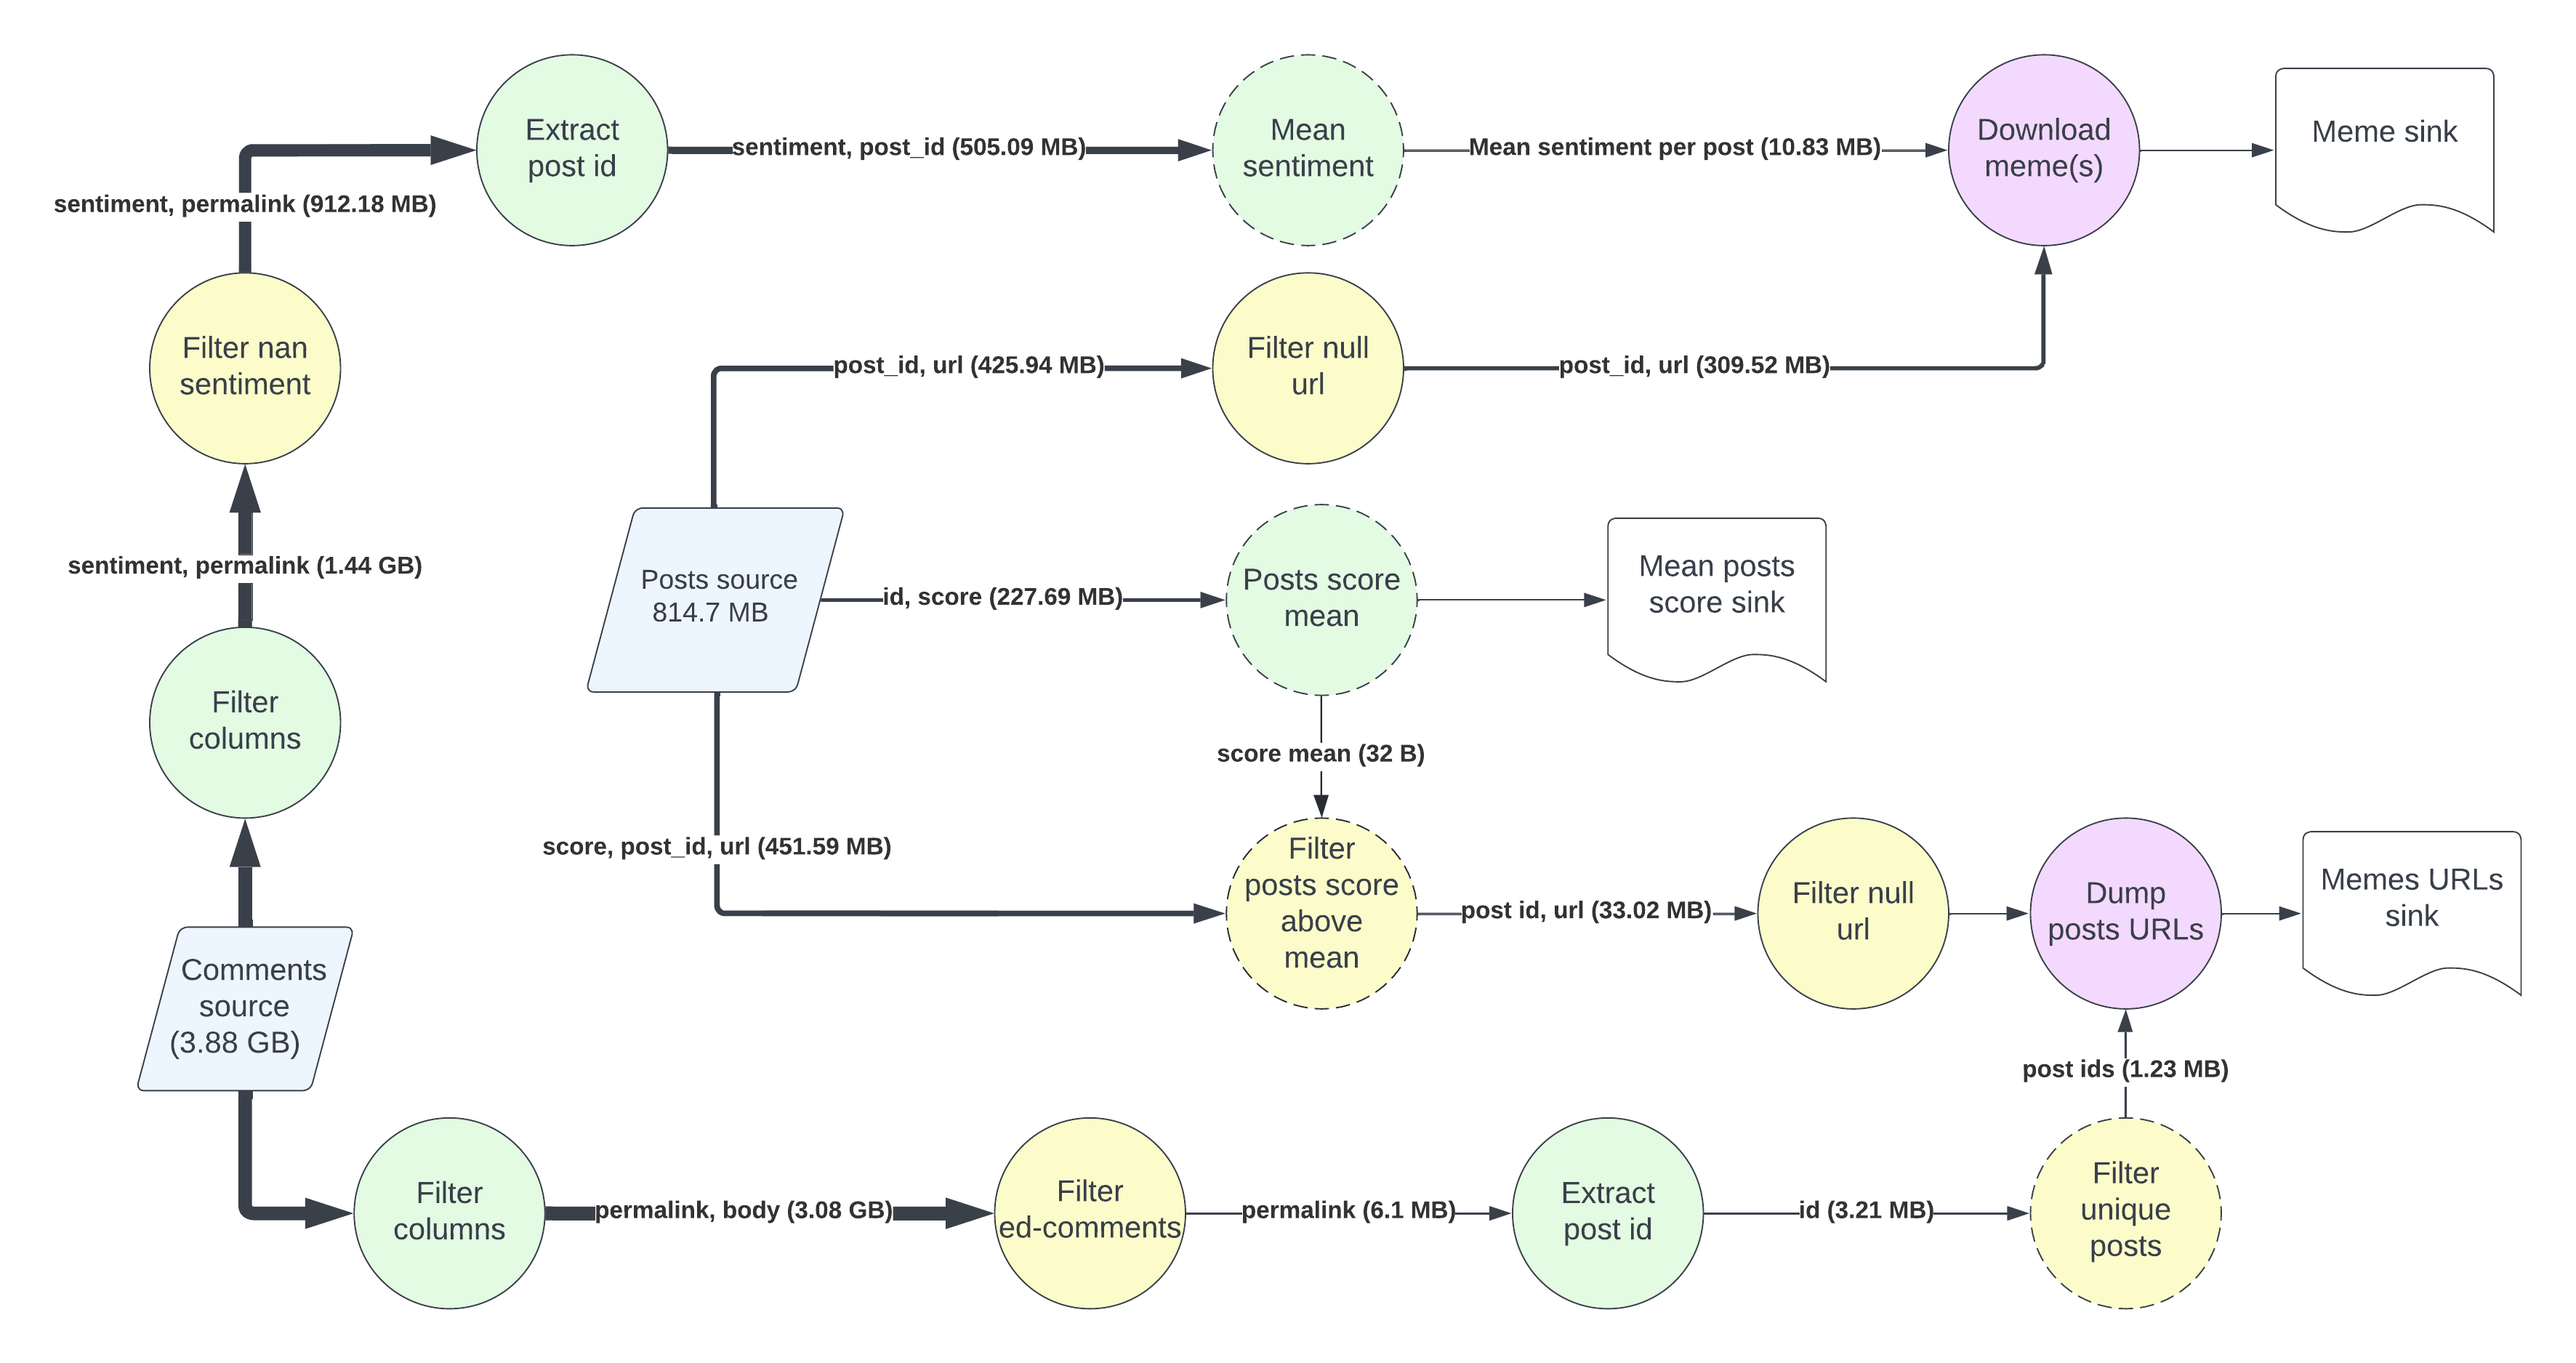
\includegraphics[width=\textwidth]{images/DAG.png}
\caption{DAG diseñado}
\end{figure}

\textbf{Nota} sobre los colores.
\begin{itemize}
	\item Rosa: \texttt{Join}
	\item Verde: \texttt{Transformation}
	\item Azul: \texttt{Source}
	\item Amarillo: \texttt{Filter}
\end{itemize}

Las líneas punteadas significan que esos nodos no son paralelizables.

\subsection{DAG Generado desde RMA}
\begin{figure}[H]
\centering
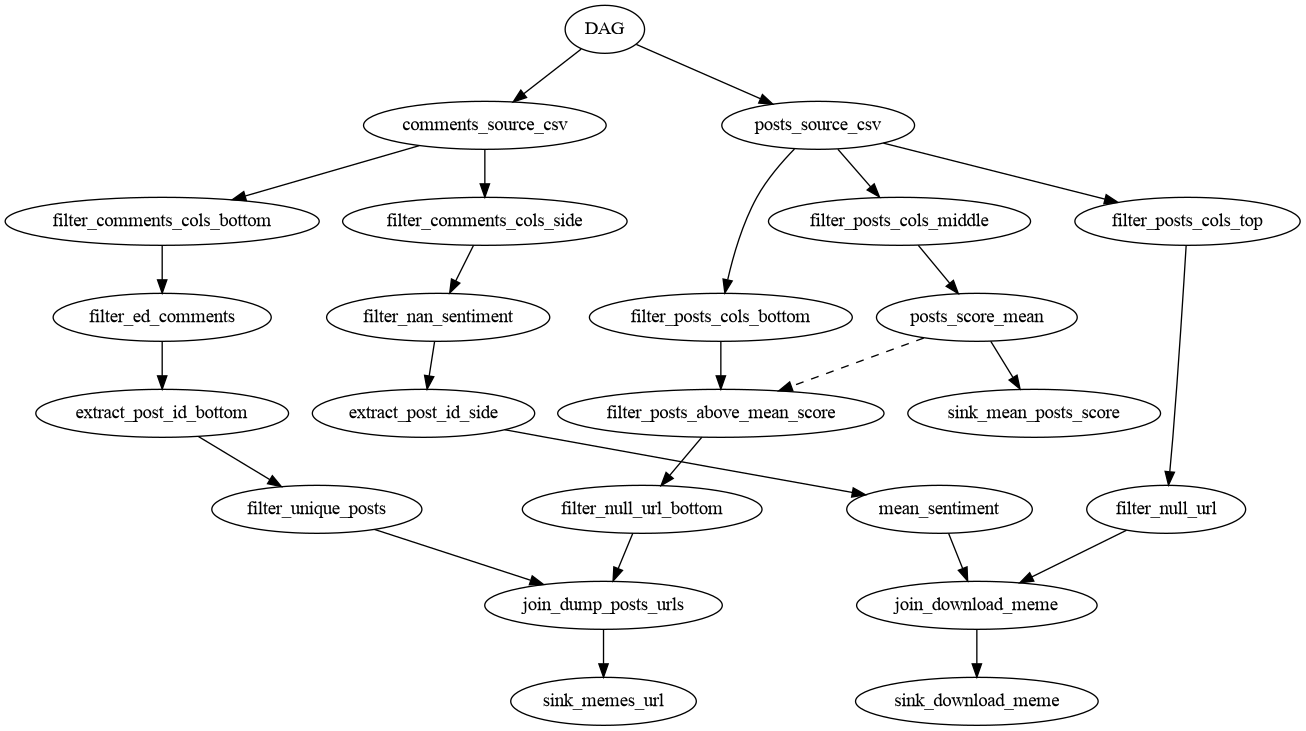
\includegraphics[width=\textwidth]{images/DAG.gv.png}
\caption{Render automático del DAG implementado.}
\end{figure}


\section{Arquitectura}
\subsection{Diagrama de Secuencia}
\begin{figure}[H]
\centering
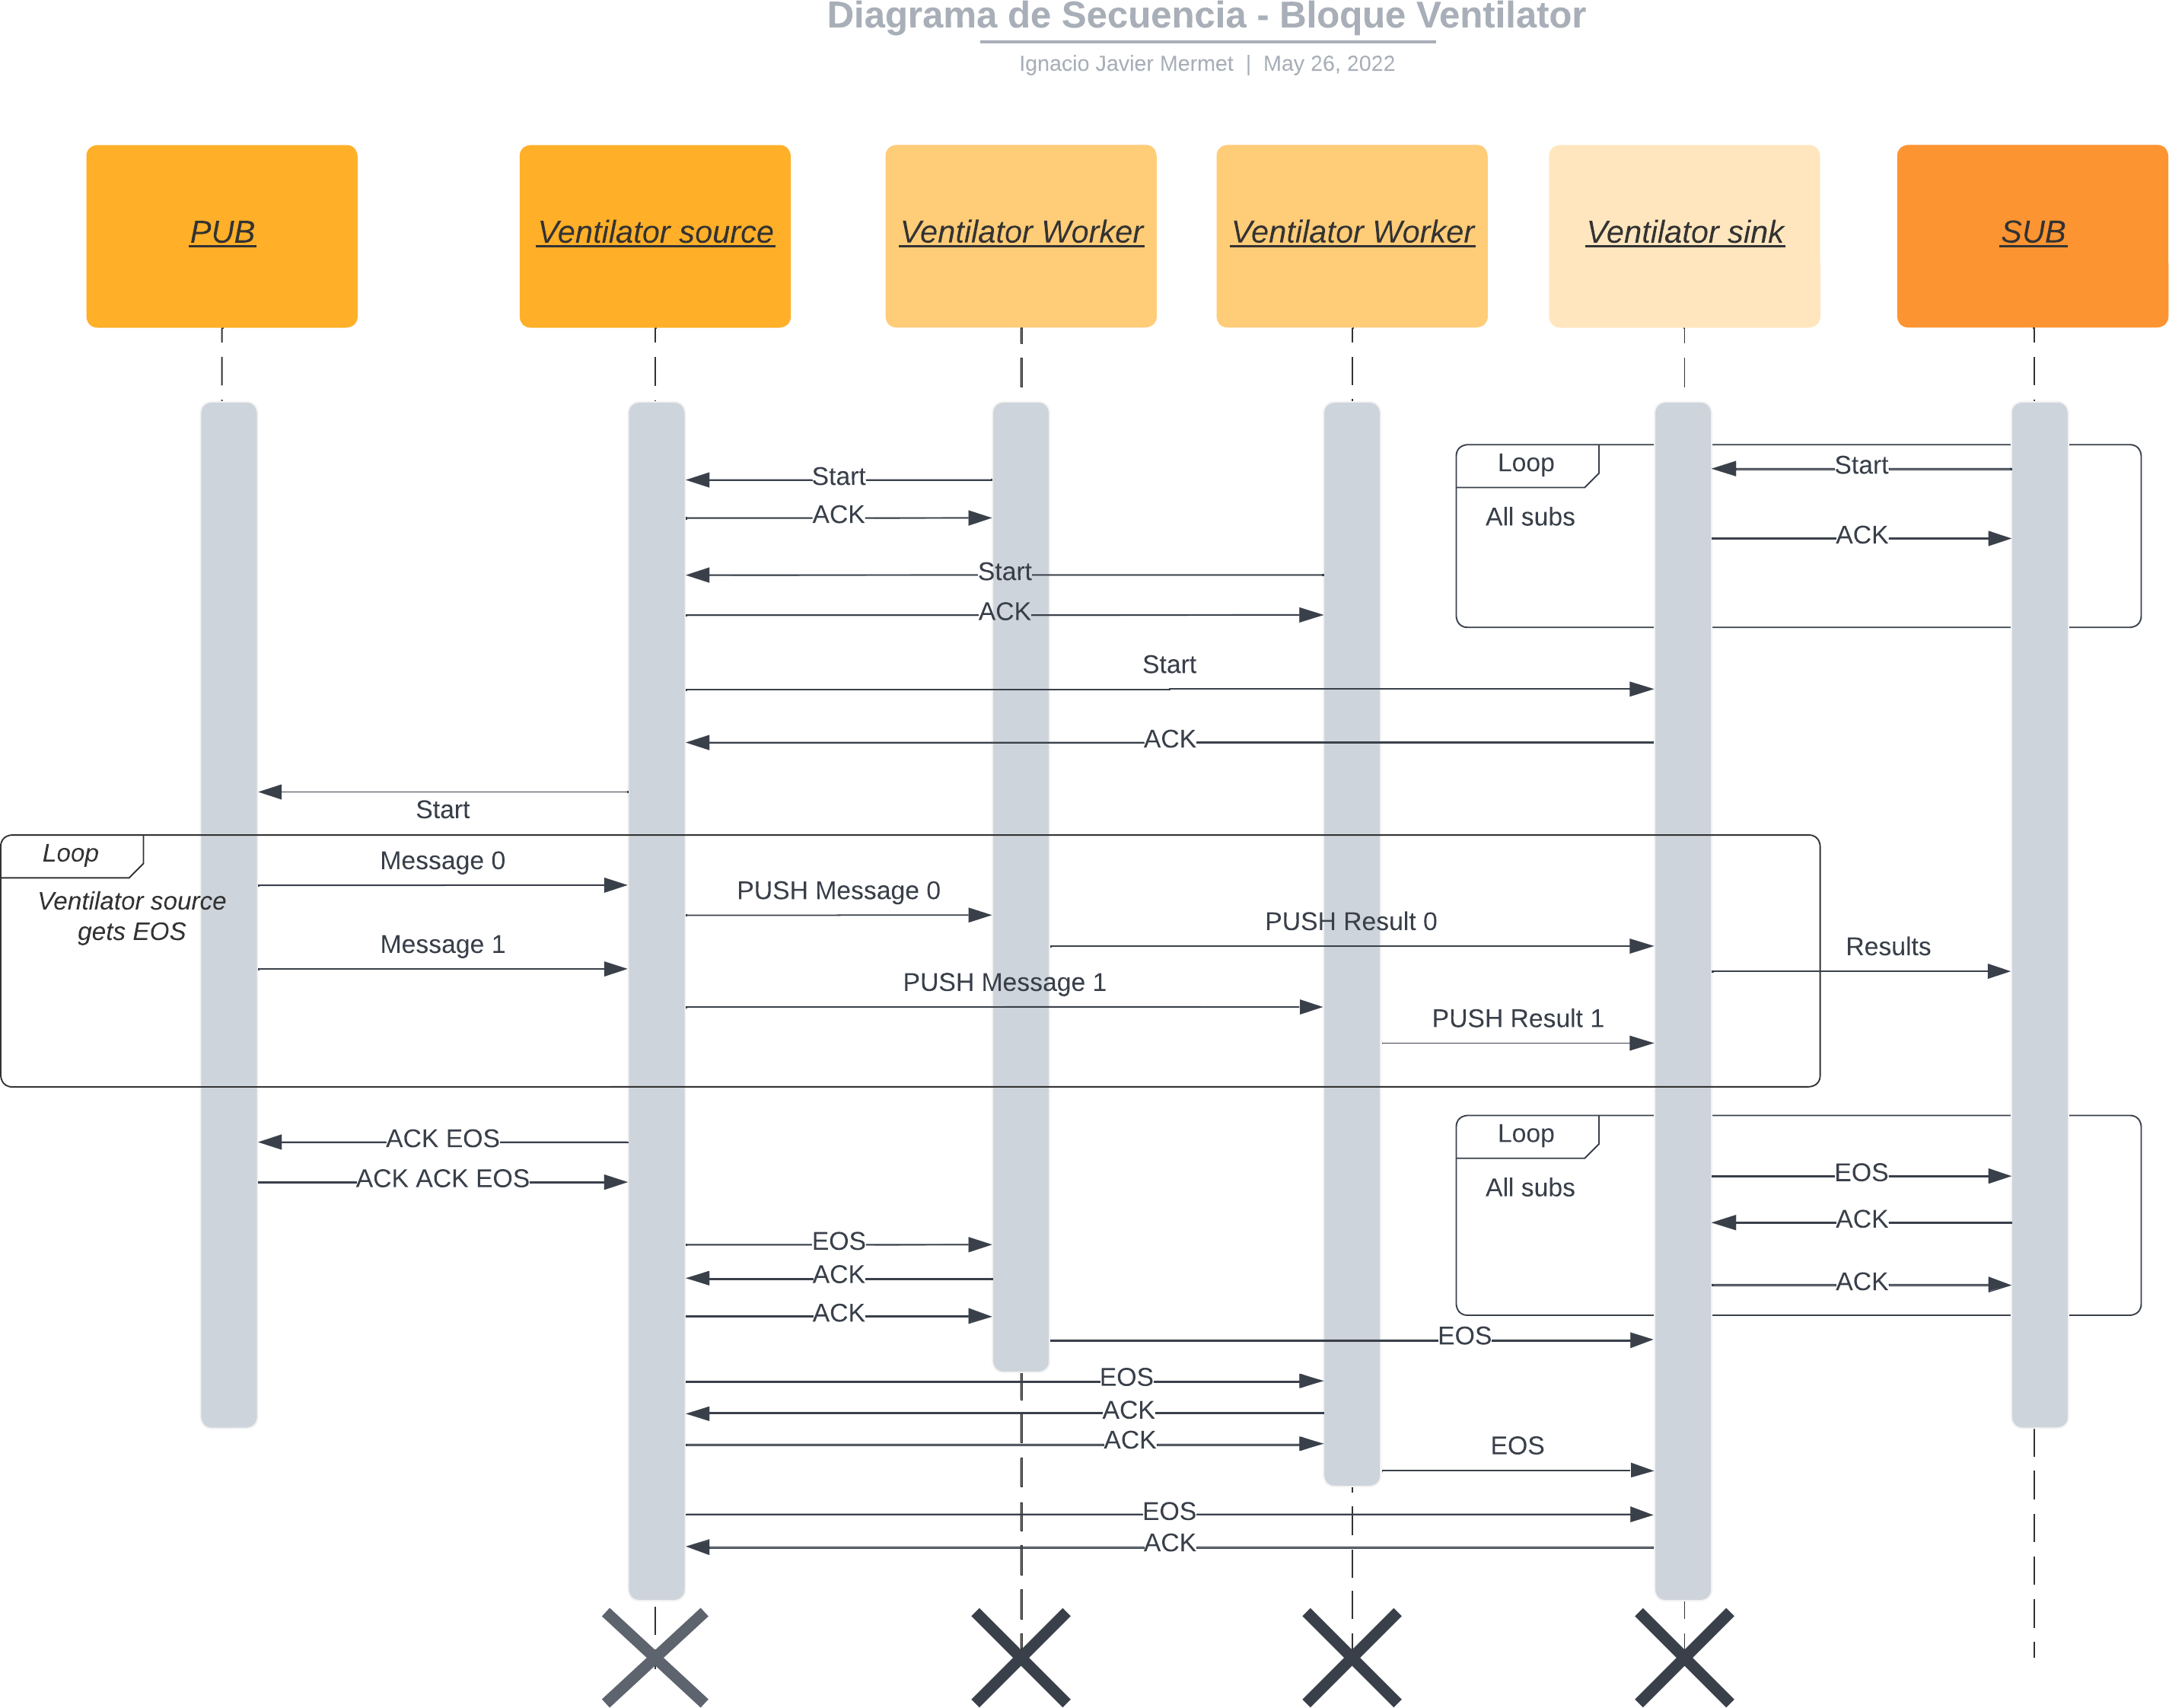
\includegraphics[width=\textwidth]{images/SequenceVentilator.png}
\caption{Diagrama de secuencia para bloques Ventilator.}
\end{figure}

\subsection{Diagrama de Robustez}
\begin{figure}[H]
\centering
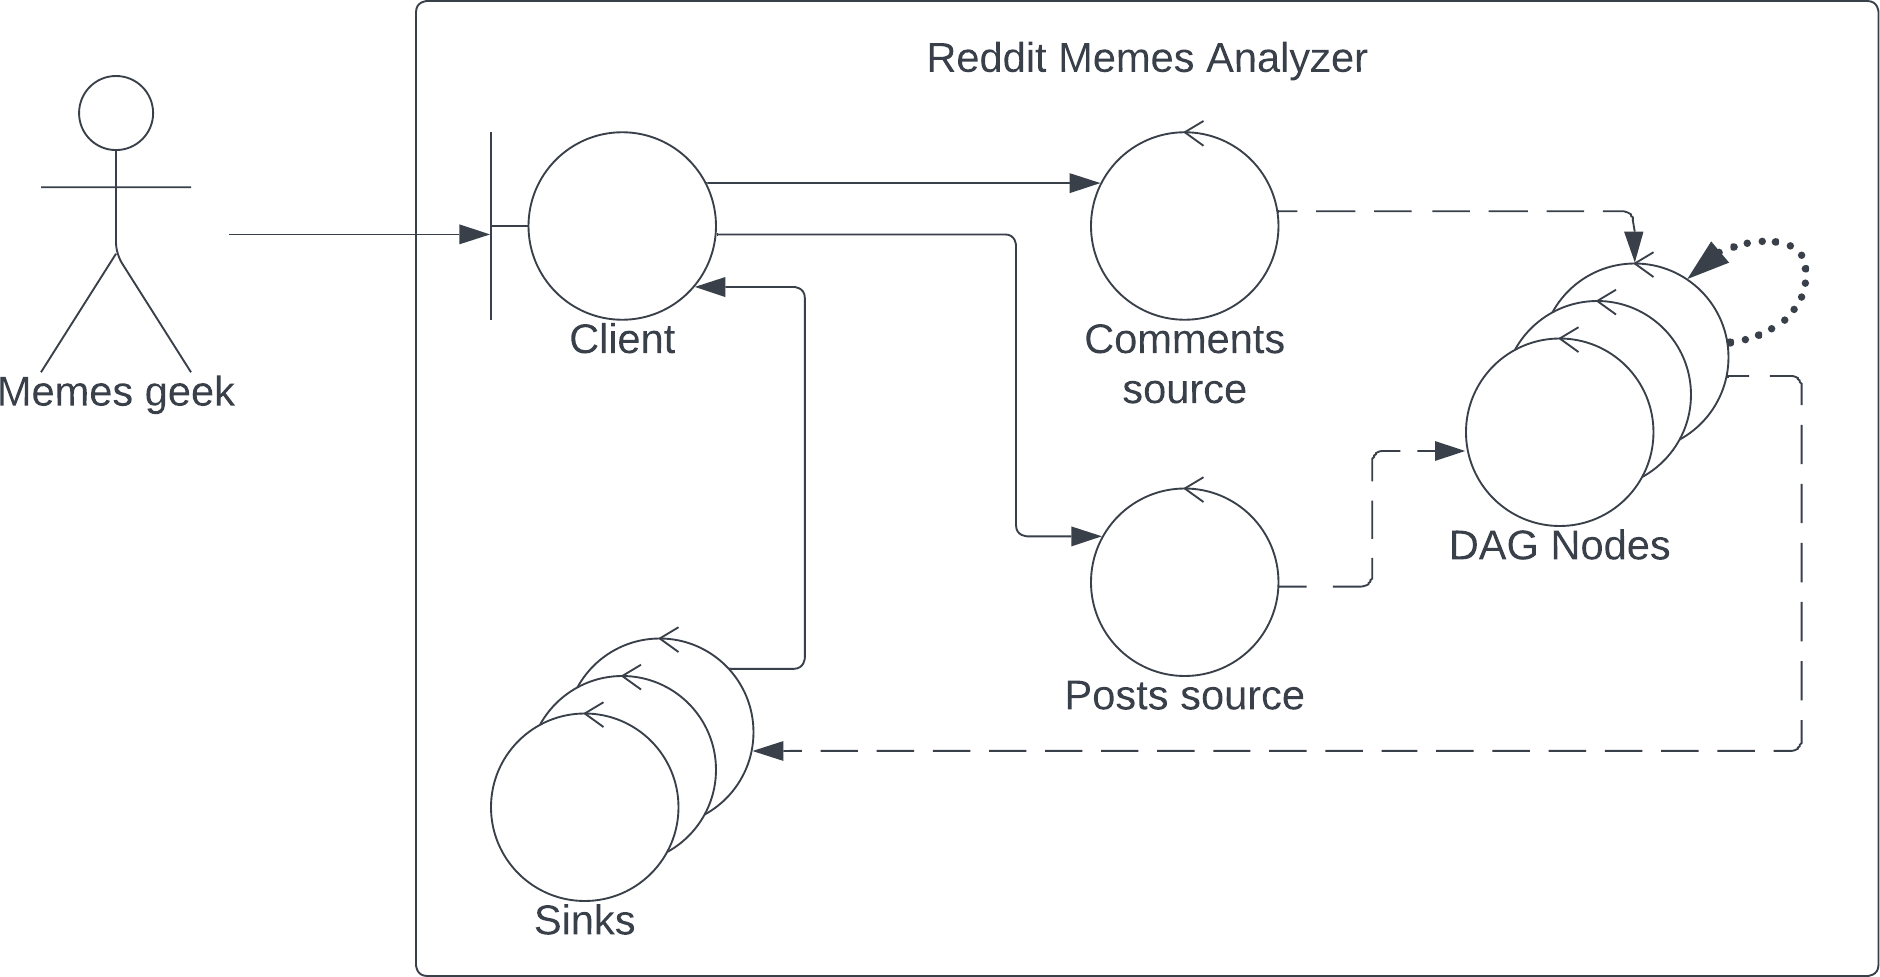
\includegraphics[width=\textwidth]{images/Robustez.png}
\caption{Diagrama de robustez.}
\end{figure}

\subsection{Diagrama de Despliegue}
\begin{figure}[H]
\centering
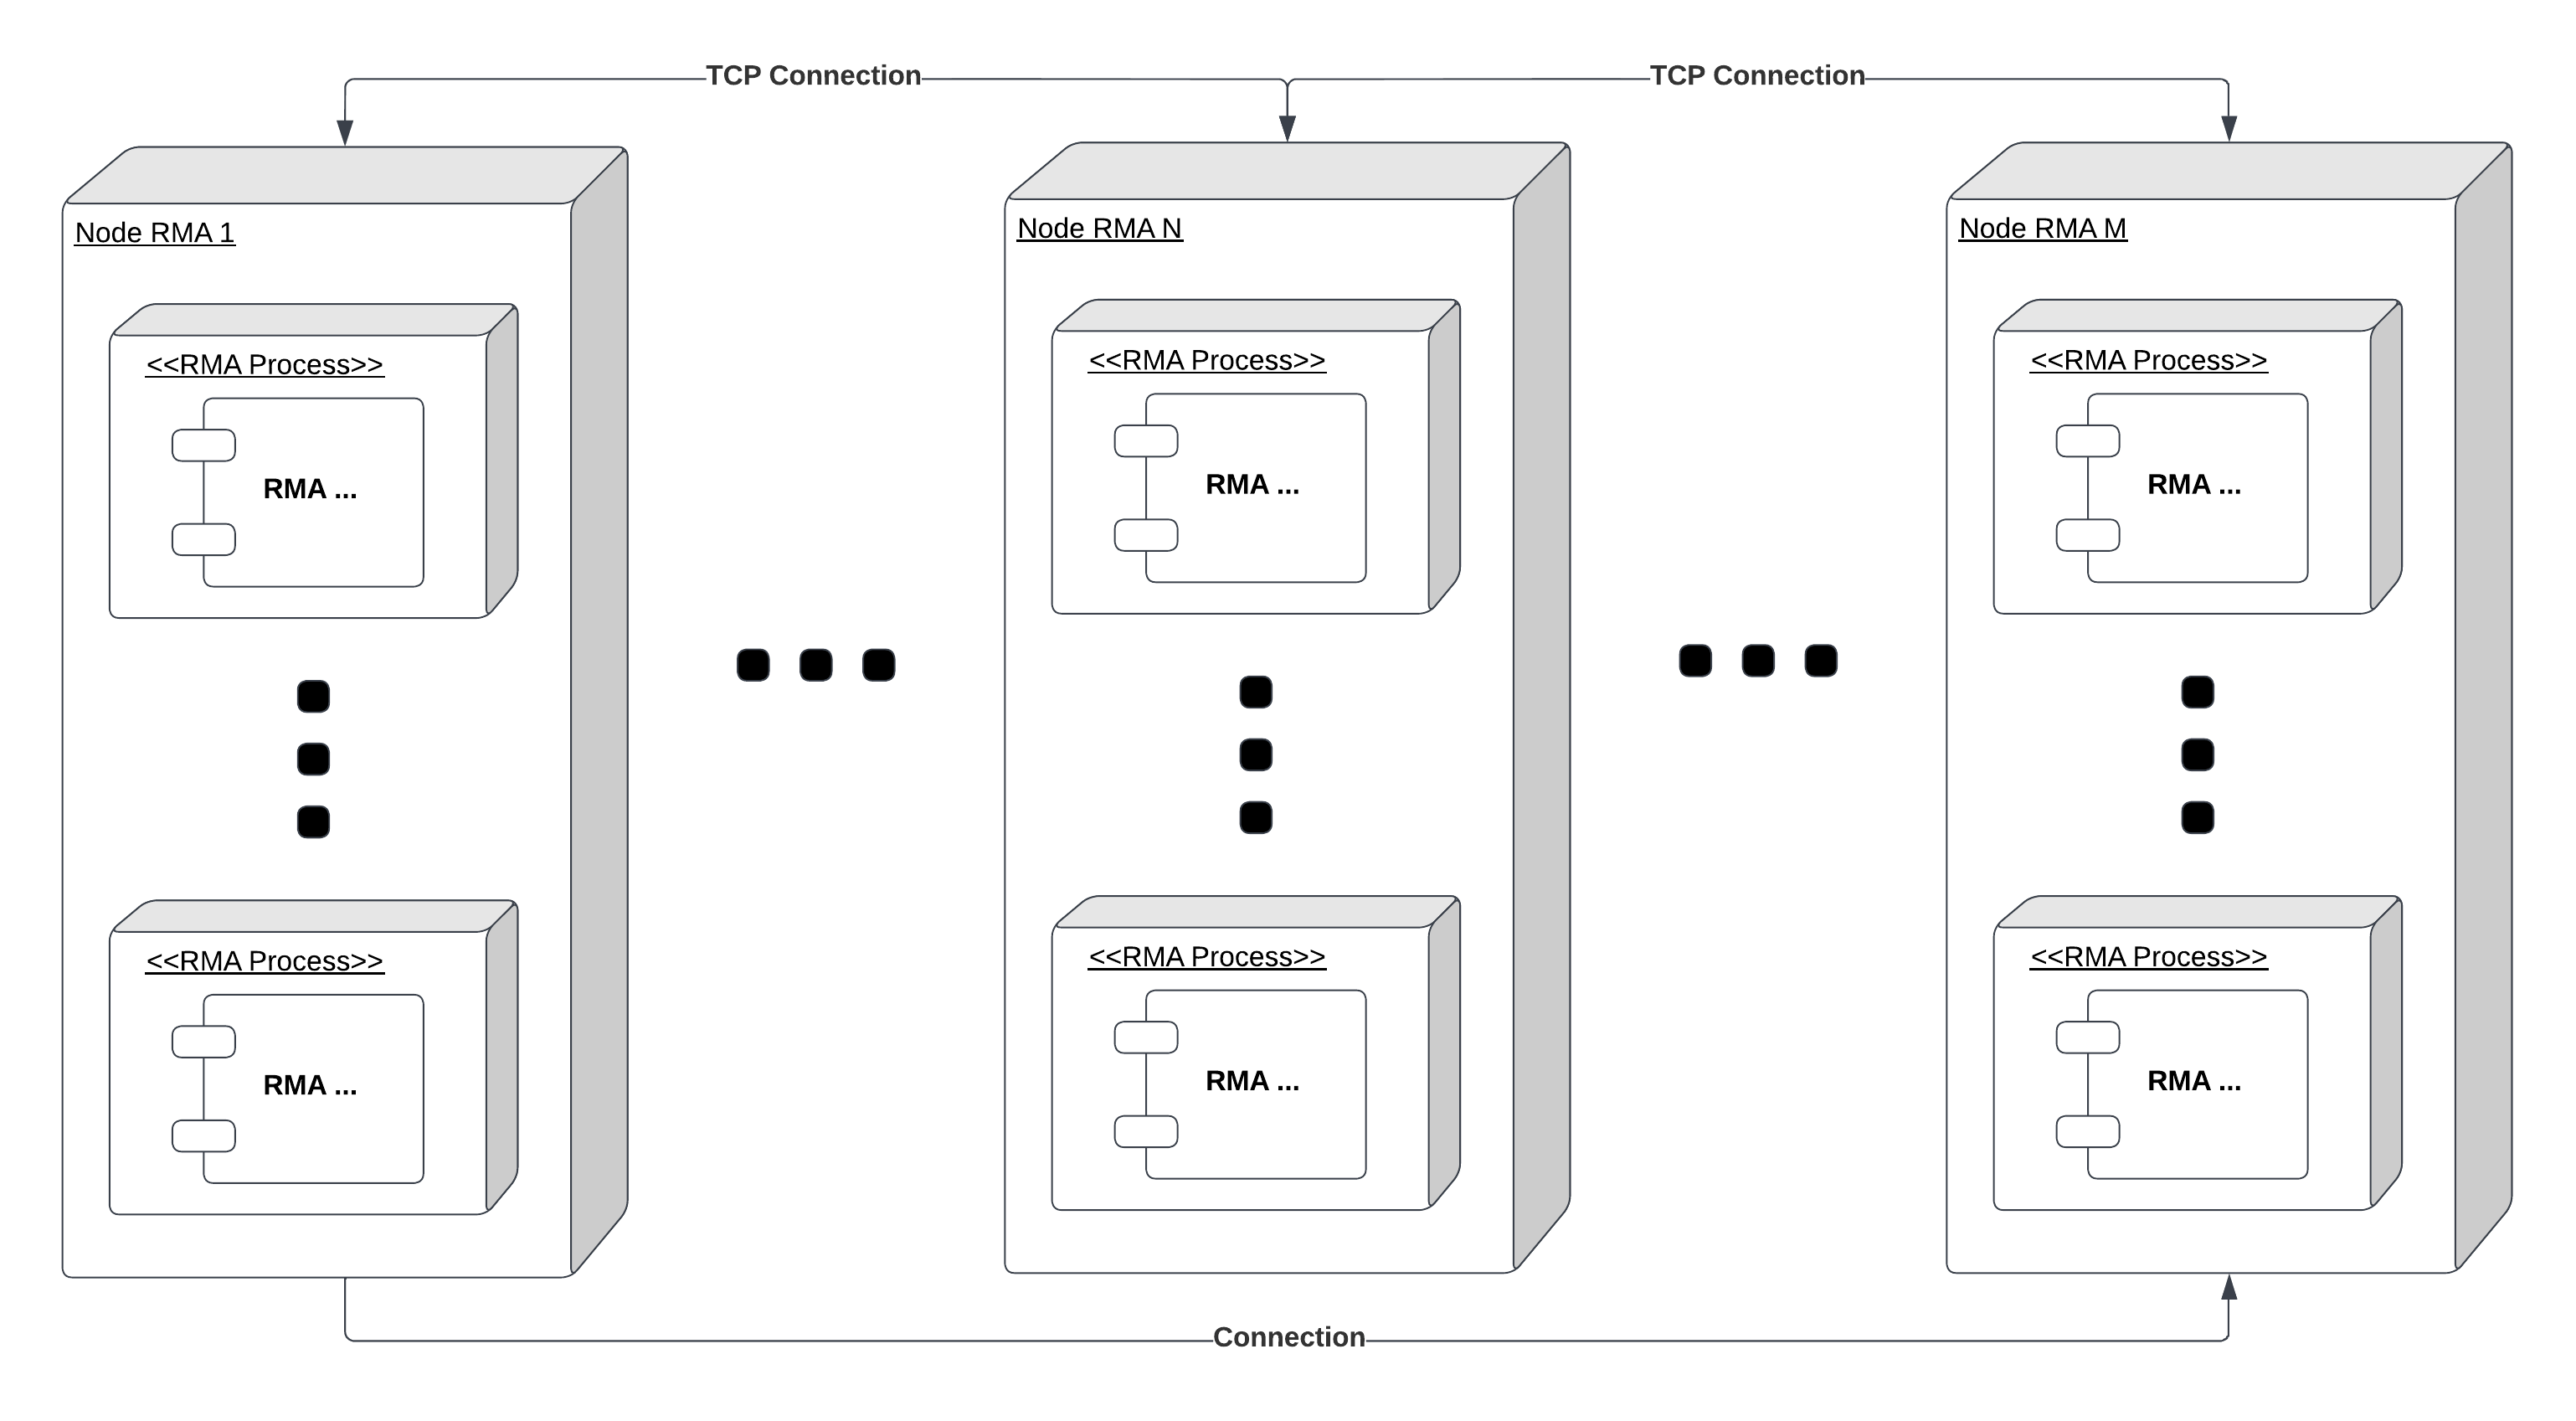
\includegraphics[width=\textwidth]{images/Despliegue.png}
\caption{Diagrama de despliegue del sistema.}
\end{figure}

\subsection{Diagrama de Paquetes}
\begin{figure}[H]
\centering
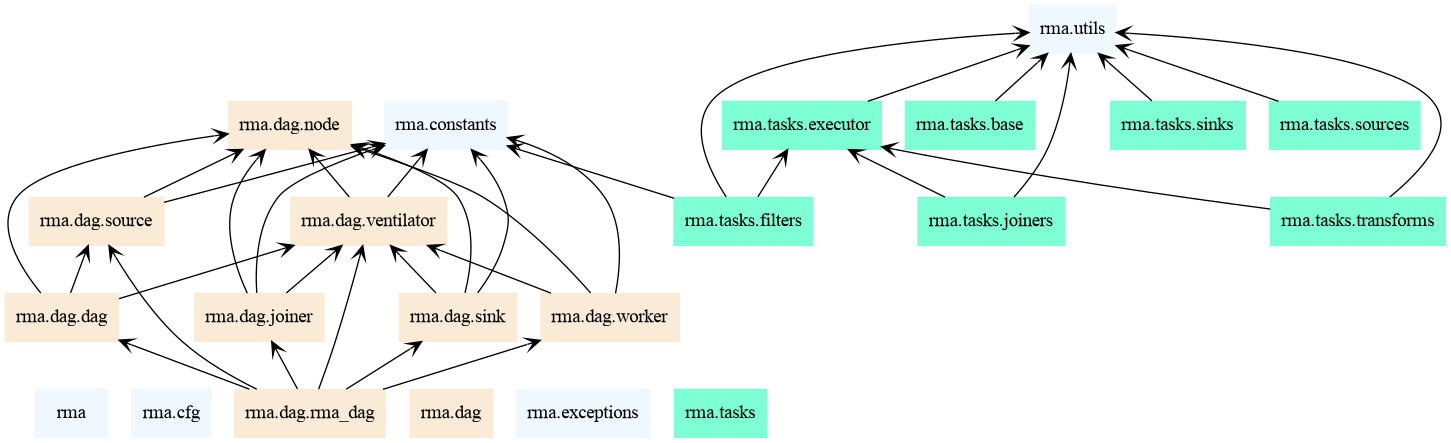
\includegraphics[width=\textwidth]{images/packages.png}
\caption{Diagrama de paquetes generado con \texttt{pyreverse}.}
\end{figure}

\section{Componentes}
\digraph{structs}{
    rankdir=TB;
    splines=polyline;
    node [shape=Mrecord];
    source [label="{Source | {<pub>PUB | <rep>REP}}"];
    ventilator_src [color=blue,label="{{<sub>SUB||<req_in>REQ}|{Ventilator|<req_out>REQ}|{<push>PUSH|<rep>REP}}"];
    ventilator_w1 [color=blue,label="{{<pull>PULL|<req>REQ}|Worker|<push>PUSH}"];
    ventilator_w2 [color=blue,label="{{<pull>PULL|<req>REQ}|Worker|<push>PUSH}"];
    ventilator_w3 [color=blue,label="{{<pull>PULL|<req>REQ}|Worker|<push>PUSH}"];
    ventilator_sink [color=blue,label="{{<pull>PULL|<rep_in>REP}|Sink|{<pub>PUB|<rep_out>REP}}"];
    worker [label="{{<sub>SUB|<req>REQ}|Worker|{<pub>PUB|<rep>REP}}"];
    sink [label="{{<sub>SUB|<req>REQ}|{Sink}}"];

    source:pub -> ventilator_src:sub;
    ventilator_src:req_in -> source:rep;

    ventilator_src:req_out -> ventilator_sink:rep_in;

    ventilator_src:push -> ventilator_w1:pull;
    ventilator_src:push -> ventilator_w2:pull;
    ventilator_src:push -> ventilator_w3:pull;

    ventilator_w1:req -> ventilator_src:rep;
    ventilator_w2:req -> ventilator_src:rep;
    ventilator_w3:req -> ventilator_src:rep;

    ventilator_w1:push -> ventilator_sink:pull;
    ventilator_w2:push -> ventilator_sink:pull;
    ventilator_w3:push -> ventilator_sink:pull;

    ventilator_sink:pub -> worker:sub;
    worker:req -> ventilator_sink:rep_out;

    worker:pub -> sink:sub;
    sink:req -> worker:rep;
}


\printbibliography

\end{document}
